\documentclass[%
  reprint,
  superscriptaddress,
  showpacs,
  showkeys,
  amsmath,amssymb,
  pra,
  longbibliography,
  floatfix,
  x11names
]{revtex4-2}

\usepackage{amsmath}
\usepackage{amssymb}
\usepackage{amsthm}
\usepackage{bm} % bold math
\usepackage{graphicx}
\usepackage{tikz}
\usetikzlibrary{decorations.markings,lindenmayersystems}
\usepackage{pgfplots}
\pgfplotsset{compat=1.18}
\usepackage{orcidlink}
\usepackage{hyperref}

\newtheorem{theorem}{Theorem}
\newtheorem{corollary}[theorem]{Corollary}

% --- DEFINITIONS FOR FIGURES (MUST BE IN PREAMBLE) ---

% Configuration parameters for Menger Sponge
\definecolor{cubeface1}{RGB}{180,180,180}  % Right face
\definecolor{cubeface2}{RGB}{220,220,220}  % Top face
\definecolor{cubeface3}{RGB}{140,140,140}  % Front face
\definecolor{cubeedge}{RGB}{80,80,80}      % Edge color

\newcommand\mengersponge[2][]{
    \pgfkeys{
        /menger/.cd,
        draw edges/.initial=true,
        edge width/.initial=0.1pt,
        .unknown/.style={\pgfkeyscurrentname/.style={#1}}
    }
    \pgfkeys{/menger/.cd, #1}

    \pgfmathsetmacro\level{int(#2 - 1)}
    \ifnum \level = 0 \relax
        \mengercube
    \else
        \begin{scope}[scale=0.333333]
            \foreach \x in {-2,0,2} {
                \foreach \y in {-2,0,2} {
                    \foreach \z in {-2,0,2} {
                        \pgfmathsetmacro{\skipthis}{
                            (\x==0 && \y==0) || (\x==0 && \z==0) || (\y==0 && \z==0) ? 1 : 0
                        }
                        \ifnum\skipthis=0
                            \begin{scope}[shift={(\x,\y,\z)}]
                                \mengersponge[#1]{\level}
                            \end{scope}
                        \fi
                    }
                }
            }
        \end{scope}
    \fi
}

\newcommand\mengercube{
    \filldraw[
        fill=cubeface1,
        draw=cubeedge,
        line width=\pgfkeysvalueof{/menger/edge width}
    ] (1,1,1) -- (1,1,-1) -- (1,-1,-1) -- (1,-1,1) -- cycle;
    \filldraw[
        fill=cubeface2,
        draw=cubeedge,
        line width=\pgfkeysvalueof{/menger/edge width}
    ] (1,1,1) -- (1,1,-1) -- (-1,1,-1) -- (-1,1,1) -- cycle;
    \filldraw[
        fill=cubeface3,
        draw=cubeedge,
        line width=\pgfkeysvalueof{/menger/edge width}
    ] (1,1,1) -- (1,-1,1) -- (-1,-1,1) -- (-1,1,1) -- cycle;
}

% Koch curve
\pgfdeclarelindenmayersystem{Koch curve}{
  \rule{F -> F+F--F+F}
}

% Cantor set
\pgfdeclarelindenmayersystem{Cantor set}{
  \rule{F -> FfF}
  \rule{f -> fff}
}
% --- END OF FIGURE DEFINITIONS ---

\begin{document}

\title{Holes Repel: Anti-Gravity as a Generic Consequence of Underdensities in a Background Substratum}

\author{Karl Svozil\,\orcidlink{0000-0001-6554-2802}}
\email{karl.svozil@tuwien.ac.at}
\homepage{http://tph.tuwien.ac.at/~svozil}
\affiliation{Institute for Theoretical Physics, TU Wien, Wiedner Hauptstrasse 8-10/136, 1040 Vienna, Austria}

\date{\today}

\begin{abstract}
Once space is modeled as a background substratum of uniform positive energy density $\rho_0$, the gravitational repulsion sometimes invoked under the heading of ``anti-gravity'' becomes a generic and unexotic phenomenon: in the Newtonian and linearized-gravity regimes, any localized region from which substratum is absent acts, relative to the background, as a negative effective mass and produces repulsive accelerations on test bodies in its exterior. The apparent negativity is a renormalization artifact of background subtraction, structurally identical to the construction that produces the Casimir energy, the effective mass of holes in a filled electronic band, and the peculiar gravity of cosmological voids; no energy conditions of the fundamental substratum are violated. We prove a universality theorem: in the Newtonian/linearized regime, the leading exterior field of a hole depends only on its volume, with shape information---fractal dimension, lacunarity, topology---entering only through subleading multipoles suppressed by $(\mathcal{R}/r)^2$. In the exact relativistic treatment we distinguish a Lorentz-scalar substratum (exterior Schwarzschild--de Sitter, static configurations requiring an Israel thin shell) from a dust-like substratum (exterior FLRW, hole as a Lema\^itre--Tolman--Bondi void), and we resolve the Bondi runaway via an Archimedean argument: the hole is buoyantly pushed away from any positive mass while the positive mass is gravitationally repelled by the hole, yielding mutual repulsion rather than runaway pursuit. The Menger sponge serves only as a visualization: at leading order any hole repels identically.
\end{abstract}

\keywords{anti-gravity, background substratum, cosmological voids, induced gravity, Menger sponge, Schwarzschild--de Sitter, Israel junction conditions}

\maketitle

\section{Introduction}
\label{sec:intro}

The notion of a gravitationally repulsive ``negative mass'' has a long and uncomfortable history in general relativity (GR). Bondi's classical analysis~\cite{bondi-1957} showed that a fundamental matter field with negative inertial mass leads to runaway pair acceleration and other pathologies, and the standard energy conditions~\cite{hawking-ellis,wald-1984} explicitly forbid such matter at the level of the stress-energy tensor. As a result, repulsive solutions of the Einstein equations---most notably the negative-mass Schwarzschild geometry---are typically regarded as mathematical curiosities devoid of physical realization.

The purpose of this paper is to argue that this judgment is, in an important sense, an artifact of insisting on a particular interpretive frame. If one abandons the picture of GR as a theory formulated on a bare manifold and instead treats space as a \emph{background substratum}---a positive-energy-density medium analogous in spirit to Einstein's 1920 reinterpretation of the ether as the metric field~\cite{einstein-aether-en} and to Sakharov's induced gravity~\cite{Sakharov-67}---then gravitational repulsion ceases to be exotic. It becomes, in the Newtonian and weak-field limits, the generic and unavoidable behavior of any localized \emph{absence} of substratum, in precisely the same sense in which a hole in a filled electronic band carries an effective positive charge and an effective negative mass~\cite{kittel-ssp,ashcroft-mermin}, in which Dirac's hole theory of the positron arises as an absence in a filled negative-energy sea~\cite{dirac-1930}, and in which a cosmological void exhibits measurable repulsive peculiar accelerations relative to the cosmic mean~\cite{shethvdw-2004,hamaus-2014}.

The thesis we wish to defend can be stated in a single sentence:

\begin{quote}
\emph{Holes repel.} A localized region from which a positive-energy substratum has been removed acts gravitationally, relative to the unperturbed background, as a source of negative effective mass and produces repulsive accelerations on test bodies in its exterior, regardless of the shape, internal structure, fractal dimension, or topology of the removed region.
\end{quote}

This claim is, on closer inspection, neither speculative nor original at the level of physical content. What is novel here is the reframing: the recognition that three superficially disparate phenomena---the Casimir effect, the negative effective mass of band holes, and the peculiar gravity of cosmic voids---share a common mathematical structure, and that this structure suffices to remove the air of pathology surrounding gravitationally repulsive solutions whenever a background is available to subtract.

We make this case in stages. In Sec.~\ref{sec:substratum} we state the substratum hypothesis and distinguish two physically inequivalent versions of it---a Lorentz-scalar (vacuum-energy-like) substratum and a frame-fixing (dust-like) substratum---both of which support the central thesis but lead to different exact relativistic geometries. Section~\ref{sec:newtonian} establishes the thesis in the Newtonian limit by direct application of the shell theorem to a background-subtracted negative source. Section~\ref{sec:relativistic} treats the relativistic version with proper care: we derive the exterior geometry for both substratum types (Schwarzschild--de Sitter for the Lorentz-scalar case; a different geometry for the dust case) and treat the hole boundary using the Israel junction conditions, which require either an explicit thin shell or a non-static dynamical boundary. Section~\ref{sec:universality} states and proves a universality theorem, valid in the Newtonian/linearized regime, to the effect that the leading exterior field of a hole depends only on its volume; this is the technical core of the paper, and it explains in what precise sense the shape of the absence---fractal or otherwise---is irrelevant. Section~\ref{sec:menger} presents the Menger sponge as an illustrative example, chosen for its visual clarity but not for any essential role in the physics. Section~\ref{sec:exotic} confronts the energy-condition and Bondi-runaway objections, the latter being resolved by an Archimedean buoyancy argument that yields mutual repulsion between hole and positive mass without invoking any pathological dynamics. We conclude in Sec.~\ref{sec:discuss}.

\section{Two versions of the substratum hypothesis}
\label{sec:substratum}

By a \emph{background substratum} we mean the hypothesis that the spatial sections of spacetime are filled, at all points, by a background field of positive energy density $\rho_0 > 0$. Two physically distinct realizations of this hypothesis are relevant for what follows, and they must be carefully distinguished, as they lead to different exact relativistic geometries even though they yield identical predictions in the Newtonian and linearized regimes.

\subsection{Type A: Lorentz-scalar substratum}
\label{sec:typeA}

The first realization assumes that the substratum is a Lorentz scalar---it has no preferred frame and looks the same to all inertial observers. The most general stress-energy tensor compatible with local Lorentz invariance is proportional to the metric,
\begin{equation}
T^{(0)}_{\mu\nu} = -\rho_0\, g_{\mu\nu},
\label{eq:T0_lorentz}
\end{equation}
which corresponds to a perfect fluid with energy density $\rho_0$ and pressure $p_0 = -\rho_0$. This is mathematically identical to a positive cosmological constant
\begin{equation}
\Lambda = \frac{8\pi G \rho_0}{c^2}.
\label{eq:Lambda_def}
\end{equation}
A Lorentz-scalar substratum is therefore equivalent, at the level of classical GR, to a vacuum-energy / dark-energy contribution. It is not ``ponderable matter'' in the conventional sense---it has negative pressure---but it is a positive-energy background in the sense relevant for our construction, and the apparent paradox in the terminology reflects the fact that a Lorentz-invariant background \emph{cannot} have ordinary mechanical pressure.

\subsection{Type B: Frame-fixing dust-like substratum}
\label{sec:typeB}

The second realization assumes that the substratum is a pressureless dust-like fluid,
\begin{equation}
T^{(0)}_{\mu\nu} = \rho_0\, u_\mu u_\nu,
\label{eq:T0_dust}
\end{equation}
where $u^\mu$ is a timelike unit vector field defining a preferred local rest frame. Such a substratum breaks local Lorentz invariance at the level of the background but does not source any anisotropic pressure, and its gravitational behavior in the Newtonian limit reduces to that of cold dust. This realization is the appropriate analogue of the cold dark matter (CDM) component in cosmology, where the cosmic rest frame is selected by the matter distribution itself, and it provides the closest physical correspondence to the cosmological-void analogy that anchors the empirical part of our discussion.

\subsection{What both versions share}

In either version, the substratum is taken to be locally removable. By a \emph{hole} we mean a bounded region $\Omega \subset \mathbb{R}^3$ within which the substratum is absent ($T_{\mu\nu} = 0$), surrounded by an exterior in which $T_{\mu\nu} = T^{(0)}_{\mu\nu}$. The microphysical mechanism that maintains this configuration is left unspecified, in the same spirit as one specifies a charge distribution in electrostatics without inquiring into the binding forces.

The background-subtracted effective stress-energy
\begin{equation}
T^{\mathrm{eff}}_{\mu\nu}(\mathbf{x}) = T_{\mu\nu}(\mathbf{x}) - T^{(0)}_{\mu\nu}
\label{eq:Teff_def}
\end{equation}
vanishes outside the hole and equals $-T^{(0)}_{\mu\nu}$ inside. We emphasize once more that this negativity is a property of the \emph{difference} field $T^{\mathrm{eff}}_{\mu\nu}$, not of any fundamental matter field. The underlying substratum has $\rho \geq 0$ everywhere; the apparent negative density inside $\Omega$ is the bookkeeping consequence of measuring deviations from a positive baseline.

In the Newtonian and linearized-GR regimes, only the energy-density component $\rho^{\mathrm{eff}} = -\rho_0\, \chi_\Omega(\mathbf{x})$ sources the gravitational field, and Type A and Type B substrata yield identical predictions. In the exact (nonlinear) relativistic regime, the difference between the two types becomes important, as discussed in Sec.~\ref{sec:relativistic}.

\section{The Newtonian argument}
\label{sec:newtonian}

The simplest and most transparent form of the thesis lives in Newtonian gravity, where it reduces to a one-line application of the shell theorem and is independent of the choice between Type A and Type B substrata.

Let $\Omega \subset \mathbb{R}^3$ be a bounded region of volume $V(\Omega)$ from which substratum of uniform density $\rho_0$ has been removed, and consider a test body at position $\mathbf{r}$ outside the convex hull of $\Omega$. The Newtonian potential generated by the effective mass distribution $\rho^{\mathrm{eff}}(\mathbf{x}) = -\rho_0\, \chi_\Omega(\mathbf{x})$, where $\chi_\Omega$ is the indicator function of $\Omega$, is
\begin{equation}
\Phi(\mathbf{r}) = -G \int_\Omega \frac{\rho^{\mathrm{eff}}(\mathbf{x})}{|\mathbf{r} - \mathbf{x}|}\, d^3x = +G\rho_0 \int_\Omega \frac{d^3x}{|\mathbf{r} - \mathbf{x}|}.
\label{eq:phi_int}
\end{equation}
The corresponding gravitational acceleration on a test body of mass $m$ is $\mathbf{g}(\mathbf{r}) = -\nabla \Phi(\mathbf{r})$, which by direct differentiation of Eq.~\eqref{eq:phi_int} reads
\begin{equation}
\mathbf{g}(\mathbf{r}) = -G\rho_0 \int_\Omega \frac{\mathbf{r} - \mathbf{x}}{|\mathbf{r} - \mathbf{x}|^3}\, d^3x.
\label{eq:g_int}
\end{equation}

For $|\mathbf{r}|$ large compared to the linear extent of $\Omega$, the integrand admits the standard multipole expansion. The leading term is
\begin{equation}
\Phi(\mathbf{r}) = +\frac{G \rho_0 V(\Omega)}{|\mathbf{r}|} + \mathcal{O}\!\left(\frac{1}{|\mathbf{r}|^3}\right),
\label{eq:phi_monopole}
\end{equation}
where the dipole term vanishes when the origin is chosen at the centroid of $\Omega$, and the quadrupole and higher multipoles fall off as $|\mathbf{r}|^{-(\ell+1)}$.

Equation~\eqref{eq:phi_monopole} is the entire physical content of the thesis at the Newtonian level. The potential outside the hole is positive and falls as $1/r$; the corresponding force on a test body is directed \emph{outward}, away from the hole, with magnitude
\begin{equation}
|\mathbf{g}(\mathbf{r})| = \frac{G \rho_0 V(\Omega)}{|\mathbf{r}|^2} + \mathcal{O}\!\left(\frac{1}{|\mathbf{r}|^4}\right).
\label{eq:g_monopole}
\end{equation}
The hole repels, with an effective gravitational charge
\begin{equation}
M_{\mathrm{eff}} = -\rho_0 V(\Omega),
\label{eq:Meff_volume}
\end{equation}
proportional to and opposite in sign to the mass of substratum that would have filled $\Omega$.

Three features of this result deserve emphasis. First, no assumption about the shape of $\Omega$ has entered: $V(\Omega)$ is the only attribute of the hole that controls the leading exterior field. Second, the construction is parameter-free given $\rho_0$ and $\Omega$: there is no defect-strength parameter, no microscopic length scale, and no dimensional ansatz to be fitted. Third, the same conclusion holds in linearized GR: writing $g_{\mu\nu} = \eta_{\mu\nu} + h_{\mu\nu}$ and treating $T^{\mathrm{eff}}_{\mu\nu}$ as the source of $h_{\mu\nu}$ in the de Donder gauge, the leading $h_{00}$ component reproduces $\Phi(\mathbf{r})$ as in Eq.~\eqref{eq:phi_monopole}, with the same shape independence and the same repulsive sign. The Newtonian and weak-field GR conclusions coincide because the linearization is, by construction, the regime in which background subtraction is mathematically legitimate.

\section{The relativistic argument: exact treatment}
\label{sec:relativistic}

We now turn to the exact (nonlinear) relativistic version of the problem. In contrast to the Newtonian case, the exact treatment depends in a nontrivial way on the substratum's equation of state, and it requires careful attention to the matching conditions at the boundary of the hole. Both subtleties are absent in the Newtonian/linearized analysis above, where they collapse onto the universal Eq.~\eqref{eq:Meff_volume}.

\subsection{Why one cannot simply ``subtract'' the background}
\label{sec:no_subtraction}

It is tempting to argue that, since outside the hole the spacetime is exactly the unperturbed substratum geometry, and since this geometry can be ``absorbed into a cosmological constant or Minkowski background,'' the exterior of the hole is then governed by the Schwarzschild solution with $M = M_{\mathrm{eff}} < 0$. This argument is incorrect. In nonlinear GR, all energy gravitates, and one cannot subtract stress-energy tensors and expect the corresponding exact metrics to subtract:
\begin{equation}
g^{\mathrm{full}}_{\mu\nu} - g^{(0)}_{\mu\nu} \neq g^{\mathrm{eff}}_{\mu\nu}\quad\text{(in general)}.
\label{eq:no_metric_subtraction}
\end{equation}
Background subtraction is a linearization device, valid when $h_{\mu\nu} = g^{\mathrm{full}}_{\mu\nu} - g^{(0)}_{\mu\nu}$ is small in some appropriate sense, but it is not an exact solution-generating technique. To obtain the correct exterior geometry, one must solve the Einstein equations directly with the actual stress-energy distribution---substratum outside the hole, vacuum inside---imposing appropriate matching at the boundary.

\subsection{Type A: exterior Schwarzschild--de Sitter}
\label{sec:exact_typeA}

For a Lorentz-scalar substratum (Type A, Sec.~\ref{sec:typeA}), the exterior of a spherically symmetric hole of radius $\mathcal{R}$ is filled with a stress-energy equivalent to a positive cosmological constant $\Lambda = 8\pi G \rho_0/c^2$. The most general spherically symmetric solution of the Einstein equations with cosmological constant is the Schwarzschild--de Sitter (SdS) metric~\cite{kottler-1918,wald-1984},
\begin{equation}
ds^2 = -F(r)\, c^2 dt^2 + F(r)^{-1}\, dr^2 + r^2\, d\Omega_2^2,
\label{eq:sds}
\end{equation}
with
\begin{equation}
F(r) = 1 - \frac{2 G M_{\mathrm{ext}}}{c^2 r} - \frac{\Lambda}{3} r^2.
\label{eq:F_sds}
\end{equation}
The interior of the hole ($r < \mathcal{R}$) is vacuum and is therefore exactly Minkowski space (by Birkhoff's theorem applied to the source-free interior),
\begin{equation}
ds^2 = -c^2 dt_{\mathrm{int}}^2 + dr^2 + r^2\, d\Omega_2^2.
\label{eq:interior}
\end{equation}
The mass parameter $M_{\mathrm{ext}}$ in the exterior is fixed by the Israel junction conditions at the boundary $r = \mathcal{R}$, to which we now turn.

\subsection{Israel junction conditions and the boundary shell}
\label{sec:israel}

Matching the empty interior~\eqref{eq:interior} to the SdS exterior~\eqref{eq:sds} across $r = \mathcal{R}$ requires that the induced metric be continuous and that any discontinuity in the extrinsic curvature be balanced by a thin-shell stress-energy~\cite{israel-1966,poisson-2004}. Continuity of the induced metric on the timelike hypersurface $\Sigma = \{r = \mathcal{R}\}$ is straightforward to arrange by reparametrization. The extrinsic curvature of $\Sigma$, computed from each side, is in general discontinuous, and the jump $[K_{ij}] = K^{+}_{ij} - K^{-}_{ij}$ defines a surface stress-energy tensor
\begin{equation}
S_{ij} = -\frac{c^4}{8\pi G}\left([K_{ij}] - h_{ij} [K]\right),
\label{eq:Sij}
\end{equation}
where $h_{ij}$ is the induced metric on $\Sigma$ and $[K]$ is the trace of the jump.

For a static spherical boundary at $r = \mathcal{R}$ separating Minkowski interior from SdS exterior, an explicit calculation yields a surface energy density $\sigma$ and surface tension $\theta$ on $\Sigma$~\cite{poisson-2004,visser-1995},
\begin{align}
\sigma &= -\frac{c^2}{4\pi G \mathcal{R}}\left[\sqrt{F_+(\mathcal{R})} - \sqrt{F_-(\mathcal{R})}\right],
\label{eq:sigma}\\
\theta &= -\frac{c^2}{8\pi G \mathcal{R}}\left[\frac{\mathcal{R} F_+'(\mathcal{R})/2 + F_+(\mathcal{R})}{\sqrt{F_+(\mathcal{R})}} - \frac{\mathcal{R} F_-'(\mathcal{R})/2 + F_-(\mathcal{R})}{\sqrt{F_-(\mathcal{R})}}\right],
\label{eq:theta}
\end{align}
with $F_+(r) = 1 - 2GM_{\mathrm{ext}}/(c^2 r) - \Lambda r^2/3$ and $F_-(r) = 1$. For these to vanish (no shell), one would need $F_+(\mathcal{R}) = F_-(\mathcal{R}) = 1$ and $F_+'(\mathcal{R}) = 0$, which is generically impossible: the bulk pressure jump $\Delta p = p_+ - p_- = -\rho_0 - 0 = -\rho_0$ between exterior substratum and empty interior cannot be supported by the field equations alone.

The conclusion is that a static spherical hole in a Type A substratum requires a thin shell at $r = \mathcal{R}$ carrying surface tension, with $\sigma$ and $\theta$ given by Eqs.~\eqref{eq:sigma}--\eqref{eq:theta}. In the small-hole limit $\Lambda \mathcal{R}^2 \ll 1$ and $GM_{\mathrm{ext}}/(c^2 \mathcal{R}) \ll 1$, the surface tension reduces to the Newtonian estimate $\theta \sim \rho_0 \mathcal{R}/2$, exactly as required to balance the pressure of a uniformly negative-pressure exterior against an empty interior.

The mass parameter $M_{\mathrm{ext}}$ extracted by an exterior observer at large $r$ (in the appropriate de Sitter sense, since SdS is not asymptotically flat) is
\begin{equation}
M_{\mathrm{ext}} = -\rho_0 \cdot \frac{4\pi}{3} \mathcal{R}^3 + M_{\mathrm{shell}},
\label{eq:Mext_total}
\end{equation}
where the first term is the bulk vacuum-energy deficit and $M_{\mathrm{shell}}$ is the contribution of the boundary shell. The parameter $M_{\mathrm{ext}}$ here is precisely the Schwarzschild mass parameter appearing in the metric function $F_+(r) = 1 - 2GM_{\mathrm{ext}}/(c^2 r) - \Lambda r^2/3$ of the SdS exterior~\eqref{eq:F_sds}; Eq.~\eqref{eq:Mext_total} thus fixes its value as the sum of the bulk and shell contributions. In the regime where the shell tension is dominated by the negative-pressure jump, $M_{\mathrm{shell}}$ is positive and partially compensates the bulk deficit; the net sign of $M_{\mathrm{ext}}$ depends on $\mathcal{R}$ and on the substratum parameters. Crucially, however, in the sub-cosmological regime $\Lambda \mathcal{R}^2 \ll 1$ the bulk deficit dominates, $M_{\mathrm{ext}} < 0$, and the test-body acceleration in the exterior remains repulsive at leading order, in agreement with the Newtonian Eq.~\eqref{eq:Meff_volume}.

We must therefore acknowledge that the exact static solution requires a thin shell, which is itself a stress-energy concentration of nontrivial character. However, the shell carries \emph{positive} surface energy density and ordinary tensile stress---it is not ``exotic matter'' in the sense of violating energy conditions. The physical picture is that the boundary of the hole is held in place by a balance between the inward push of the substratum's negative pressure and the outward gravitational pull of the negative effective mass. If the shell is removed, the configuration becomes dynamical: see Sec.~\ref{sec:dynamics}.

\subsection{Type B: dust-like substratum}
\label{sec:exact_typeB}

For a dust-like substratum (Type B, Sec.~\ref{sec:typeB}), the exterior stress-energy is $T^{(0)}_{\mu\nu} = \rho_0 u_\mu u_\nu$ with $u^\mu$ defining a preferred frame. The exterior geometry is no longer SdS but rather a Tolman--Bondi-type solution~\cite{tolman-1934,bondi-1947}, in which the substratum collapses (or expands) under its own gravity. There is no static exterior in this case: a uniform dust in equilibrium against its own gravity is a Friedmann-like cosmology, and the hole is then a void embedded in a Friedmann background.

This is precisely the cosmological-void setup. The exterior geometry is locally FLRW, with $H(t)$ determined by the dust density $\rho_0$, and the hole is a Lema\^itre--Tolman--Bondi (LTB) void in this background~\cite{shethvdw-2004,nadathur-2019}. The peculiar gravitational acceleration of test bodies near the void boundary, computed by background-subtracting the FLRW Hubble flow, is repulsive and has magnitude given by the linearized expression~\eqref{eq:g_monopole} to leading order. The matching at the boundary is again governed by Israel-type conditions, but now the boundary is naturally non-static (it expands with the void), and no thin shell is required: the LTB construction matches smooth dust profiles across radial shells.

The Type B realization therefore has the advantage of providing a directly observed laboratory---late-universe void cosmology---in which the substratum picture is empirically realized. Its disadvantage, relative to Type A, is that it requires a preferred frame and is therefore not a candidate for a fundamental Lorentz-invariant substratum. The two versions are best regarded as complementary: Type A as a candidate fundamental theory, Type B as a phenomenological framework with observational support.

\subsection{Dynamics of the boundary in the absence of a shell}
\label{sec:dynamics}

If no thin shell is imposed at the boundary of a Type A hole, the configuration is non-static. The negative pressure of the exterior pushes the boundary inward; the negative effective mass pushes test bodies (and, by Newton's third law applied within the substratum's degrees of freedom, the substratum itself) outward. Whether the hole expands or collapses depends on the detailed dynamical equations of the substratum, which are not specified in the present framework.

A toy model is provided by treating the substratum as a perfect fluid with $p = -\rho$ and the boundary as a freely-moving timelike hypersurface. The Friedmann-like equation for the boundary radius $\mathcal{R}(\tau)$ in the proper time of a comoving observer takes the form
\begin{equation}
\left(\frac{d\mathcal{R}}{d\tau}\right)^2 = c^2\left[\frac{2 G |M_{\mathrm{eff}}|}{c^2 \mathcal{R}} + \frac{\Lambda \mathcal{R}^2}{3} - K\right],
\label{eq:friedmann_boundary}
\end{equation}
where $K$ is a constant of integration set by initial conditions. For positive $\Lambda$ and $|M_{\mathrm{eff}}| > 0$, the right-hand side is positive and the boundary expands monotonically: an unsupported Type A hole inflates, drained outward by the exterior's negative pressure and the repulsive effective mass. The hole is therefore dynamically unstable in the static-exterior sense, but stable in the sense that it does not collapse to a singularity. This is consistent with the cosmological intuition that holes (voids) in a vacuum-energy-dominated background grow with the cosmic expansion.

For a Type B (dust) substratum, the analogue of Eq.~\eqref{eq:friedmann_boundary} reproduces the LTB void evolution, in which voids grow more slowly than the cosmic background (a phenomenon directly observed in galaxy redshift surveys~\cite{hamaus-2014,nadathur-2019}).

\section{Universality: the shape of the hole is irrelevant in the linearized regime}
\label{sec:universality}

We now formalize the shape-independence of the leading repulsive effect in the regime where it is exactly true---namely, Newtonian gravity (equivalently, linearized GR). In the exact nonlinear regime, the conclusion holds only at leading order in the multipole expansion and in the appropriate weak-field / small-hole limit; we comment on this restriction explicitly below.

\begin{theorem}[Universality of repulsion from holes; Newtonian/linearized regime]
\label{thm:universality}
Let $\Omega \subset \mathbb{R}^3$ be any bounded measurable region with finite Lebesgue measure $V(\Omega) < \infty$, and let the centroid of $\Omega$ be located at the origin. Define the hole's effective mass distribution as $\rho^{\mathrm{eff}}(\mathbf{x}) = -\rho_0\, \chi_\Omega(\mathbf{x})$, with $\rho_0 > 0$. Then in Newtonian gravity (or, equivalently, in linearized GR with weak-field source), for any $\mathbf{r}$ outside the smallest sphere containing $\Omega$, the gravitational potential generated by $\rho^{\mathrm{eff}}$ admits the multipole expansion
\begin{equation}
\Phi(\mathbf{r}) = \frac{G \rho_0 V(\Omega)}{r} + \sum_{\ell \geq 2} \frac{1}{r^{\ell+1}} \sum_{m=-\ell}^{\ell} q_{\ell m}(\Omega)\, Y_{\ell m}(\hat{\mathbf{r}}),
\label{eq:multipole}
\end{equation}
where $r = |\mathbf{r}|$, $\hat{\mathbf{r}} = \mathbf{r}/r$, $Y_{\ell m}$ are spherical harmonics, and the multipole moments
\begin{equation}
q_{\ell m}(\Omega) = -\frac{4\pi G \rho_0}{2\ell+1} \int_\Omega |\mathbf{x}|^\ell\, Y_{\ell m}^*(\hat{\mathbf{x}})\, d^3x
\label{eq:moments}
\end{equation}
encode the shape of $\Omega$. The dipole term ($\ell = 1$) vanishes by the centroid condition.
\end{theorem}

\begin{proof}
The multipole expansion of $1/|\mathbf{r} - \mathbf{x}|$ in spherical harmonics for $|\mathbf{x}| < |\mathbf{r}|$ gives
\begin{equation}
\frac{1}{|\mathbf{r} - \mathbf{x}|} = \sum_{\ell=0}^\infty \frac{4\pi}{2\ell+1} \frac{|\mathbf{x}|^\ell}{r^{\ell+1}} \sum_{m=-\ell}^{\ell} Y_{\ell m}^*(\hat{\mathbf{x}}) Y_{\ell m}(\hat{\mathbf{r}}).
\end{equation}
Inserting into Eq.~\eqref{eq:phi_int} and exchanging integration with summation (justified by absolute convergence outside the bounding sphere) yields Eq.~\eqref{eq:multipole} with the moments~\eqref{eq:moments}. The $\ell = 0$ moment evaluates to $G \rho_0 V(\Omega)$, and the $\ell = 1$ moment vanishes by definition of the centroid.
\end{proof}

\begin{corollary}
\label{cor:universality}
Let $\Omega_1$ and $\Omega_2$ be two bounded regions of equal volume $V(\Omega_1) = V(\Omega_2) = V$, with centroids at the origin and bounded by a common sphere of radius $\mathcal{R}$. Then in the Newtonian/linearized regime, for $r \gg \mathcal{R}$,
\begin{equation}
\Phi_1(\mathbf{r}) - \Phi_2(\mathbf{r}) = \mathcal{O}\!\left(\frac{\mathcal{R}^2}{r^3}\right),
\end{equation}
and in particular, the leading $1/r$ exterior fields of the two holes are identical.
\end{corollary}

\paragraph{Restriction to the linear regime.}
The proof of Theorem~\ref{thm:universality} is a Newtonian multipole expansion and uses linear superposition of the contributions from individual mass elements. This linearity is exact in Newtonian gravity and in linearized GR but fails in the nonlinear regime: the exact static exterior of a non-spherical absence in GR is not, in general, the multipole expansion of a Newtonian potential. In the nonlinear regime, asymmetric absences source gravitational radiation if they evolve dynamically, and even static asymmetric holes will produce exterior geometries that differ from the Newtonian multipole answer at higher orders in $GM/(c^2 r)$. The universality result should therefore be read as a statement about the dominant Newtonian/weak-field exterior, valid whenever $r \gg \mathcal{R}$ and $GM_{\mathrm{eff}}/(c^2 r) \ll 1$. In this regime---which covers all empirically accessible situations short of the strong-field limit---the conclusion holds: the shape of the hole is invisible at leading order.

The physical content of Theorem~\ref{thm:universality} and Corollary~\ref{cor:universality} is the following. \emph{In the regime where the linearized analysis applies, the shape of a hole is invisible at leading order in its exterior gravitational field.} A spherical cavity, a cubical cavity, a Swiss-cheese arrangement of small cavities, a random foam, and a Menger sponge of equal total absent volume all produce the same leading $1/r$ repulsive potential outside their common bounding sphere. Shape information enters only through the quadrupole and higher multipoles, which decay as $r^{-(\ell+1)}$ and become negligible at distances $r \gg \mathcal{R}$.

This universality is what justifies---and what limits---the role of the Menger sponge in the present work. It is one of infinitely many shapes that a hole can take, all of which give rise, at leading order, to identical repulsive exterior fields. The fractal dimension, lacunarity, self-similarity, and detailed topology of the absence are physically silent at the dominant order. They survive only as fingerprints in the subleading multipole structure---fingerprints that, for any fixed total absent volume, are bounded above by $(\mathcal{R}/r)^2$ corrections to the leading effect.

The corollary also explains, retroactively, why the construction in earlier formulations of this circle of ideas appears ad hoc: the elaborate parametrizations of the absence in terms of fractal dimensions and defect-strength parameters do no work that the volume of the absence does not already do.

\section{The Menger sponge as illustration}
\label{sec:menger}

For concreteness, and because it offers a striking visual realization of an absence with rich internal structure, we briefly describe the Menger sponge~\cite{Menger1926a_reprint,Edgar_ClassicsOnFractals}. The sponge is constructed by starting with a unit cube, dividing it into 27 sub-cubes, removing the central sub-cube and the six face-centered sub-cubes, and iterating this prescription on each of the 20 surviving sub-cubes ad infinitum. The resulting set is a universal curve with Hausdorff dimension $D_H = \ln 20 / \ln 3 \approx 2.7268$ and vanishing Lebesgue measure in the limit of infinite iteration.

\begin{figure}[ht]
\centering
\resizebox{.36\textwidth}{!}{
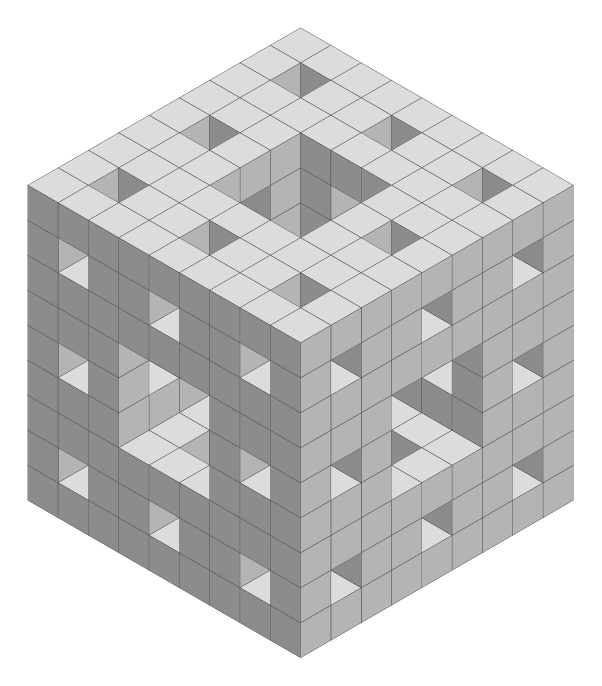
\begin{tikzpicture}[
    x={(0.866cm,-0.5cm)},
    y={(0cm,1cm)},
    z={(-0.866cm,-0.5cm)},
    scale=2
]
    \mengersponge{3}
\end{tikzpicture}
}
\caption{The Menger sponge at the third iteration. In the present framework, the visible material represents the substratum and the cavities represent the absence. By Theorem~\ref{thm:universality}, the leading exterior gravitational field of this configuration depends only on the total absent volume, in the linearized regime, and is identical to that of a single spherical cavity of equal volume.}
\label{fig:menger}
\end{figure}

A Menger-sponge-shaped absence in the substratum (Fig.~\ref{fig:menger}) is a perfectly admissible region $\Omega$ in the sense of Theorem~\ref{thm:universality}: it is bounded, measurable, and has well-defined volume at every finite iteration. At iteration $n$, the absent volume is
\begin{equation}
V_n = \mathcal{R}^3 \left[1 - \left(\tfrac{20}{27}\right)^n\right],
\label{eq:Vn}
\end{equation}
where $\mathcal{R}$ is the side length of the bounding cube. As $n \to \infty$, $V_n \to \mathcal{R}^3$: the substratum disappears entirely, leaving an absence of total volume equal to the bounding cube. The leading exterior gravitational field is then, by Theorem~\ref{thm:universality},
\begin{equation}
\Phi_\infty(\mathbf{r}) = \frac{G \rho_0 \mathcal{R}^3}{r} + \mathcal{O}(\mathcal{R}^2 / r^3),
\end{equation}
identical to the leading field of a uniform cubical absence and (to within the multipole correction) to that of a spherical absence of the same volume.

We stress what this calculation does \emph{not} show. It does not show that the fractal structure of the Menger sponge plays any role in producing the repulsion. It does not show that the Hausdorff dimension $D_H$ enters the exterior physics at any order. It does not show that the elaborate self-similar microstructure of the sponge is physically necessary, or even physically relevant, for the central thesis of the paper. The sponge serves here only as a visualizable example of an absence, chosen because absence is hard to depict and the sponge makes it easy. Any other absence of the same volume would do equally well; the cavities of the sponge are pedagogy, not physics.

\section{Why this is not exotic matter}
\label{sec:exotic}

The classical objections to gravitationally repulsive solutions in GR are of two kinds: violation of the standard energy conditions on the stress-energy tensor, and the Bondi runaway instability of negative-mass dynamics. We argue that, in the substratum framework, neither objection applies.

\subsection{Energy conditions}

The standard energy conditions are conditions on a fundamental matter field's stress-energy tensor $T_{\mu\nu}$~\cite{hawking-ellis,wald-1984,kontou-2020}. The Type A substratum stress-energy $T^{(0)}_{\mu\nu} = -\rho_0 g_{\mu\nu}$ with $\rho_0 > 0$ is mathematically equivalent to a positive cosmological constant: it satisfies the weak, dominant, and null energy conditions, but as is well known for any vacuum-energy-like contribution, it violates the strong energy condition, and indeed is the standard model of the dark-energy component driving the observed late-time cosmic acceleration~\cite{Riess1998,Perlmutter1999}. The Type B (dust) substratum satisfies all standard energy conditions including the strong one. The complementary configuration in which the substratum is absent has $T_{\mu\nu} = 0$, which trivially satisfies all the energy conditions as well. \emph{The fundamental matter content of the model satisfies the energy conditions in exactly the same sense as standard cosmological dark energy or dark matter.}

The negativity that drives the repulsion appears not in $T_{\mu\nu}$ but in the background-subtracted quantity $T^{\mathrm{eff}}_{\mu\nu} = T_{\mu\nu} - T^{(0)}_{\mu\nu}$. This object is not a fundamental stress-energy tensor; it is a difference of two physically realized stress-energies, computed for the purpose of isolating the localized gravitational effect of a deviation from a uniform background. Asking whether $T^{\mathrm{eff}}_{\mu\nu}$ satisfies the energy conditions is a category mistake of the same kind as asking whether the difference of two zero-point energy sums in the Casimir effect satisfies positivity: the difference is constructed precisely to encode the deviation from a positive baseline, and is meaningful only relative to that baseline.

The thin shell at the boundary of the hole, required by the Israel junction conditions for a Type A static configuration (Sec.~\ref{sec:israel}), carries positive surface energy density and ordinary tensile stress; it satisfies the standard energy conditions in its own right and is not exotic matter. The shell is the GR-level price of insisting on a static configuration; in the dynamical (Type B / void cosmology) picture, no such shell is required.

This is not a rhetorical move; it is the standard interpretive posture of three established subfields of physics:

\paragraph{Casimir energy.} The negative energy density between Casimir plates is the difference between two divergent vacuum sums~\cite{casimir-1948,milton-2001,bekenstein-2013}. The fundamental electromagnetic field has positive zero-point energy density everywhere; the negativity is an artifact of subtracting the unbounded plate-free vacuum from the unbounded plate-present vacuum and observing that the difference is finite and negative.

\paragraph{Effective mass of band holes.} An empty state in an otherwise filled electronic band carries an effective positive charge and an effective negative inertial mass~\cite{kittel-ssp,ashcroft-mermin}. These are properties of the \emph{absence} relative to the filled-band background; the underlying electrons have ordinary positive mass and negative charge throughout. Dirac's hole theory of the positron~\cite{dirac-1930} is the relativistic analogue.

\paragraph{Peculiar gravity in cosmological voids.} An underdense region of the late universe gravitates repulsively relative to the cosmic mean density. This is observed in the form of measured outflow velocities of galaxies near void boundaries~\cite{shethvdw-2004,hamaus-2014,nadathur-2019}, and is computed routinely in cosmological perturbation theory by background-subtracting the FLRW mean from the local density. This is precisely the Type B realization of our framework, and provides its strongest empirical anchor.

\subsection{The Bondi runaway and the Archimedean resolution}
\label{sec:archimedes}

Bondi's classical argument~\cite{bondi-1957} considers a pair of fundamental masses, one positive and one negative, both treated as autonomous dynamical point particles obeying $\mathbf{F} = m \mathbf{a}$ with their respective signed inertial masses. The negative mass is gravitationally repelled by the positive mass while gravitationally attracted to it (because $-m \cdot \mathbf{F}_{\mathrm{attractive}} =$ acceleration in the $+\mathbf{F}$ direction, but with reversed kinematic effect once $m < 0$). The pair accelerates indefinitely in the same direction, violating any sensible notion of dynamical stability.

In the substratum framework, the resolution of this paradox is not philosophical but mechanical, and it follows from elementary fluid mechanics. Consider a positive mass $M_+$ placed at finite distance from a hole of effective mass $M_{\mathrm{eff}} = -|M_{\mathrm{eff}}| < 0$. There are two physical effects, which must be analyzed together:

\emph{(i) Gravitational force on the positive mass due to the hole.} Treating the hole as a static negative effective source, the positive mass experiences a gravitational acceleration directed \emph{away} from the hole, of magnitude $G|M_{\mathrm{eff}}|/r^2$ at separation $r$. The positive mass is repelled.

\emph{(ii) Buoyant force on the hole due to the positive mass.} The substratum surrounding the hole is gravitationally attracted toward $M_+$. As the substratum accelerates toward $M_+$, the absence of substratum---the hole---is buoyantly displaced in the \emph{opposite} direction, by precisely the same Archimedean mechanism that causes a bubble in water to rise against gravity. Let $\hat{\mathbf{n}}$ denote the unit vector pointing from the hole toward $M_+$. The substratum at the hole's location is gravitationally accelerated toward $M_+$ with $\mathbf{g}_{\mathrm{at\ hole}}(M_+) = +(GM_+/r^2)\hat{\mathbf{n}}$, and the hole, as a buoyant absence, acquires the opposite acceleration:
\begin{equation}
\mathbf{a}_{\mathrm{hole}} = -\mathbf{g}_{\mathrm{at\ hole}}(M_+) = -\frac{G M_+}{r^2}\, \hat{\mathbf{n}}.
\label{eq:archimedes}
\end{equation}
The minus sign expresses that the hole accelerates \emph{away} from $M_+$.

The two effects therefore agree in direction: the positive mass and the hole accelerate \emph{away from each other}. This is not the Bondi runaway, in which the two objects accelerate in the same direction with the negative-mass partner ``chasing'' the positive one indefinitely. It is, instead, ordinary mutual repulsion, of the same sign as electrostatic repulsion between like charges, with momentum and energy supplied by the substratum's gravitational interaction with $M_+$.

The Bondi paradox arises from treating the negative-mass object as an autonomous Newtonian particle with intrinsic negative inertia. In the substratum framework, the hole is not such a particle: it is a buoyant displacement in a fluid background, and its dynamics are governed by the Archimedean response of the surrounding substratum. The hole has no intrinsic inertia of its own; it inherits its dynamical response from the substratum it displaces.

This is physically the same mechanism that governs the dynamics of a semiconductor hole in an electric field. A hole experiences a force opposite to that on the surrounding electrons, and accelerates accordingly with effective negative mass---but at no point is there a runaway, because the dynamics are determined by the (positive-mass, positive-charge-magnitude) electrons of the filled band, not by an autonomous negative-mass particle. Dirac's hole-theoretic positron exhibits the same well-behaved dynamics for the same reason.

We conclude that the standard objections to negative-mass Schwarzschild solutions, and to gravitational repulsion more generally, do not apply to holes in a background substratum. The repulsion is real, calculable, and exotic only in the precise sense in which Casimir energy, semiconductor holes, and cosmic voids are exotic---which is to say, not exotic at all.

\section{Discussion}
\label{sec:discuss}

We have argued that gravitational repulsion is a generic and unexotic phenomenon once space is modeled as a background substratum, with two important qualifications relative to the most naive form of the claim. First, the exact relativistic geometry depends on the substratum's equation of state, and a careful treatment requires either a Lorentz-scalar substratum (whose exterior is Schwarzschild--de Sitter and whose hole boundary requires an Israel-type thin shell) or a frame-fixing dust-like substratum (whose exterior is FLRW and whose hole is a Lema\^itre--Tolman--Bondi void, dynamically evolving without any thin shell). Second, the universality theorem---that the shape of the hole is invisible at leading order---is exact only in the Newtonian/linearized regime. In the nonlinear regime, asymmetric holes generate non-Schwarzschild multipole structure in their exteriors and, if dynamical, gravitational radiation; the universality result then degrades to a leading-order statement about the dominant $1/r$ Newtonian piece, which remains shape-independent.

What remains, after these qualifications, is the principal substantive claim: in the regime where the linearized analysis applies---which covers essentially all empirically accessible situations short of the strong-field limit---a hole in a positive-energy substratum produces a repulsive $1/r$ potential whose magnitude is fixed by the absent volume and whose sign is fixed by the act of background subtraction. The negativity is a renormalization artifact, not a fundamental pathology; the energy conditions of the underlying substratum are nowhere violated; and the Bondi runaway instability is replaced, via Archimedean buoyancy, by ordinary mutual repulsion. The Menger sponge with which we began plays no essential role in this physics: at leading order, the volume of the absence is everything, and the fractal structure---or any other shape detail---is invisible.

The principal universality result has a methodological consequence worth stating explicitly. Earlier formulations of the present circle of ideas attached considerable interpretive weight to the fractal character of the absent region: Hausdorff dimensions, defect-strength parameters, and microscopic length scales were invoked to fix the magnitude of the effective mass. Theorem~\ref{thm:universality} shows that, in the linearized regime, this interpretive apparatus is unnecessary. The leading exterior field of any bounded hole is fixed by its volume alone; the fractal, foamy, or smooth character of the absence enters only through subleading multipoles. The Menger sponge is a vivid illustration of an absence with intricate internal structure, but its intricacy is gravitationally inert at the leading order.

Several limitations of the present framework deserve acknowledgment.

\emph{The substratum is hypothetical.} We have not derived the existence of a substratum from any deeper principle, nor have we proposed a microphysical model of it. The substratum hypothesis is offered here as an interpretive posture in which gravitational repulsion becomes natural; whether such a substratum exists is a separate empirical question. The Type B (dust) realization is closest to observational reality, since the late-universe matter distribution does play the role of a substratum in the precise sense relevant for void cosmology; the Type A (Lorentz-scalar) realization is closer to a candidate fundamental theory, identified with the cosmological-constant component of the dark sector.

\emph{The boundary requires care.} As emphasized in Sec.~\ref{sec:israel}, a static Type A hole requires a thin shell at its boundary, with surface tension determined by the substratum's negative pressure. This shell is not exotic matter, but it is a stress-energy concentration that must be included in any honest accounting of the configuration's energy budget. In the dynamical (Type B / void) picture, the boundary evolves smoothly without any shell, and the framework reduces to the well-developed LTB void cosmology.

\emph{The universality is linearized.} The shape-independence of the leading repulsion is exact only in the Newtonian/linearized regime. Strong-field generalizations would require the construction of explicit non-spherical exact solutions of the Einstein equations with absent matter, and we make no such construction here.

\emph{Observational signatures.} The cleanest observational test of the substratum picture would be the detection of compact objects with anomalously repulsive gravitational fields: defocusing rather than focusing gravitational lensing, anomalous Shapiro time advances rather than delays, or systematic outward perturbations on test-body trajectories. None of these has been observed at sub-cosmological scales. At cosmological scales, the repulsive peculiar gravity of voids \emph{is} observed and constitutes the closest existing empirical realization of the substratum picture; whether it can be extended to compact astrophysical objects is an open question.

A natural extension of the present work is to ask whether the substratum framework offers a fresh perspective on the late-time accelerated expansion of the universe~\cite{Riess1998,Perlmutter1999}. If the universe is filled with a Type A substratum and its large-scale structure is dominated by underdense voids, then the framework presented here predicts that void-dominated regions repel each other, which on cosmological scales contributes additively to a positive cosmological constant in a void-rich cosmography. We do not pursue this connection here, but note it as a direction in which the substratum picture might make contact with observational cosmology beyond the level of analogy.

In summary: in the regime where the linearized analysis applies, holes repel, generically, at leading order, independently of their shape. This is not a new mathematical fact---it is shell theorem, Birkhoff (applied to the source-free interior), and multipole expansion applied to a background-subtracted source---but it is, we believe, a useful reframing of what gravitational repulsion is and why it should not be regarded as exotic. The Menger sponge with which we began serves only to remind the eye that absence can have structure; the physics, at leading order, sees only the absence.

\begin{acknowledgments}
The author thanks an anonymous referee for incisive criticism of an earlier version of this manuscript, in particular for emphasizing the misapplication of Birkhoff's theorem to a non-vacuum exterior, the necessity of treating the boundary via the Israel junction conditions, the distinction between Lorentz-scalar and dust-like substrata, and the Archimedean resolution of the Bondi runaway, all of which substantially shaped the present version.

This text was partially created and revised with assistance from large language models. All content, ideas, and prompts were provided by the author.

This research was funded in whole or in part by the Austrian Science Fund (FWF) Grant DOI: 10.55776/PIN5424624. The author acknowledges TU Wien Bibliothek for financial support through its Open Access Funding Programme.
\end{acknowledgments}

\bibliography{svozil}

\end{document}
